\documentclass[10pt]{standalone}
\usepackage[utf8]{inputenc}
\usepackage{pgf,tikz,pgfplots}
\pgfplotsset{compat=1.15}
\usepackage{mathrsfs}
\usetikzlibrary{arrows}
\pagestyle{empty}
\begin{document}
\definecolor{zzttqq}{rgb}{0.6,0.2,0.}
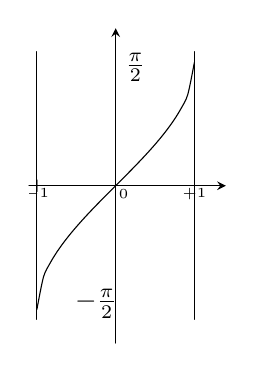
\begin{tikzpicture}[line cap=round,line join=round,>=triangle 45,x=1.0cm,y=1.0cm]
\begin{axis}[
x=1.0cm,y=1.0cm,
axis lines=middle,
ymajorgrids=false,
xmajorgrids=false,
xmin=-1.1,
xmax=1.4,
ymin=-2,
ymax=2,
%xtick={-1.0,0.0,...,1.0},
%ytick={-1.5707963267948966,0.0,...,1.5707963267948966},
xticklabels=\empty,
yticklabels=\empty,
ytick=\empty]
\clip(-1.1,-1.7) rectangle (1.5,1.7);
\draw[domain=-1.00:1.00] plot[smooth]({\x},{rad(asin(\x))});
\draw (1.,-1.698702015445294) -- (1.,1.7022109964648522);
\draw  (-1.,-1.698702015445294) -- (-1.,1.7022109964648522);
\begin{scriptsize}
\draw (0.25,1.5)node {$ \frac{\pi}{2}$};
\draw (-0.25,-1.5)node {$-\frac{\pi}{2}$};
\draw (-1.,-0.1)node {{\tiny\ensuremath -1}};
\draw (1.,-0.1)node {{\tiny\ensuremath +1}};
\draw (0.1,-0.1)node {{\tiny\ensuremath 0}};
\end{scriptsize}
\end{axis}
\end{tikzpicture}
\end{document}